\renewcommand{\hostname}{example}
\renewcommand{\os}{Linux OS Soft XP}
\renewcommand{\ip}{42.42.42.42}
\renewcommand{\tcpports}{1,2,3}
\renewcommand{\udpports}{23,42}
\renewcommand{\vuln}{CVE-123-42 "`Stupid Idiot User"'}
%Just choose one , comment out the other
\toggletrue{priv}
%\togglefalse{priv}

%--------------------------------------------------------------------------------------------------------------------
 
%---------------------------------------Start writing here-------------------------
\section{\hostname}
\subsection{Enumeration}

	\label{tab:\hostname}
\begin{longtable}{|c|c|}
\caption{Service enumeration \hostname}\\
\hline
\multicolumn{2}{|c|}{\textbf{\hostname}}\\
\hline
\hline
Type&open ports\\
\hline
TCP&\tcpports{}\\
\hline
UDP&\udpports{}\\

\hline
\hline
\multicolumn{1}{|c|}{\textbf{\os}}&\multicolumn{1}{|c|}{\textbf{\ip}}\\
\hline


\end{longtable}
\subsection{Exploitation}

\subsubsection{Used Vulnerability: \vuln}
abc
\subsubsection{Vulnerability Explanation:}
BLA BLA WRITE SOMETHING HERE 


%please insert also the priv esc. cmmands in this block. Right now the files don't work as intended. If you need you can use also the post block .. just the if clause for the images don't like the code enviroment.
\begin{lstlisting}[caption={Exploitation of \hostname},label=\hostname-exploit]
*@Kali prep:@*

*@Modifications in the exploit@*

*@Running the exploit@*

*@Escaping the low priv shell:@*
\end{lstlisting}


\begin{figure}[!ht]
\centering
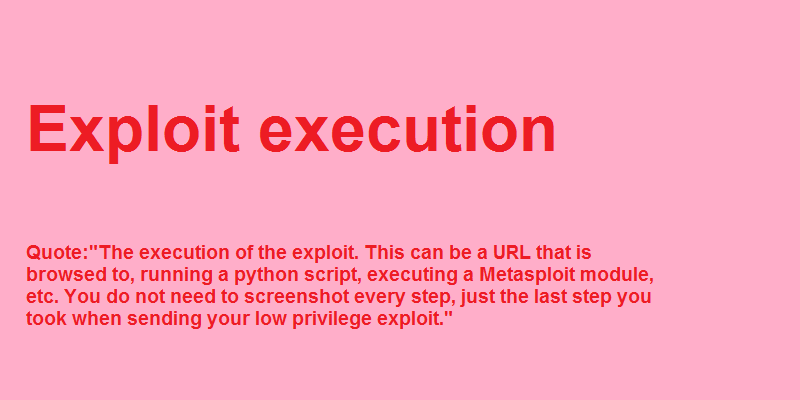
\includegraphics [width=\textwidth]{./hosts/\hostname/exploitexecution.png}
%scale 0.5 bedeutet 50% der originalgröße
%angle=90 Grafik um 90° drehen
\caption[Exploitation of \hostname]{Exploitation of \hostname} \label{\hostname-1}
\end{figure}


  \iftoggle{priv}
    {
   

%Conditional Privilege Escalation Block .. --------------------------------------------------------------------------------------------------------------------

\FloatBarrier

%Part for Priv escalation -------------------------------------------------------------------------------------------
\subsubsection{Privilege Escalation}




\begin{figure}[!ht]
\centering

\includegraphics [width=\textwidth]{./hosts/\hostname/local.png}
%scale 0.5 bedeutet 50% der originalgröße
%angle=90 Grafik um 90° drehen
\caption[Local shell of \hostname]{Local shell of \hostname} \label{\hostname-2}
\end{figure}


\begin{figure}[!ht]
\centering
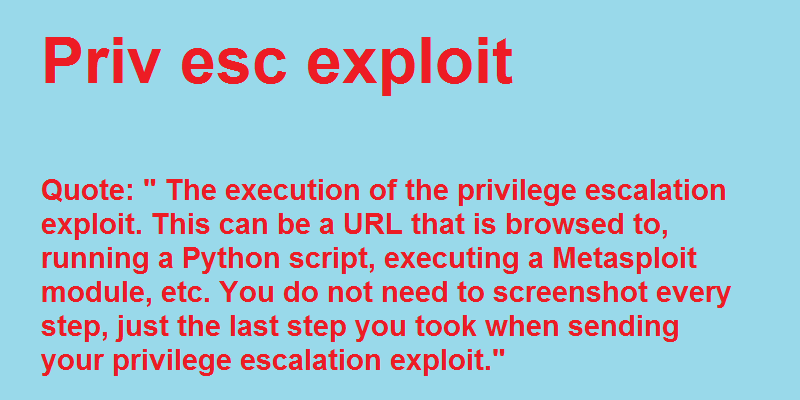
\includegraphics [width=\textwidth]{./hosts/\hostname/privescexploit.png}
%scale 0.5 bedeutet 50% der originalgröße
%angle=90 Grafik um 90° drehen
\caption[Priv escalation exploit of \hostname]{Priv escalation exploit of \hostname} \label{\hostname-3}
\end{figure}

}
{}
%--------------------------------------End of Priv Esc Block------------------------
\FloatBarrier
\subsubsection{Proof and Post escalation}
\begin{lstlisting}[caption={Post exploitation of \hostname},label=\hostname-post]
*@Post exploitation commands run:@*

\end{lstlisting}

\begin{figure}[!ht]
\centering
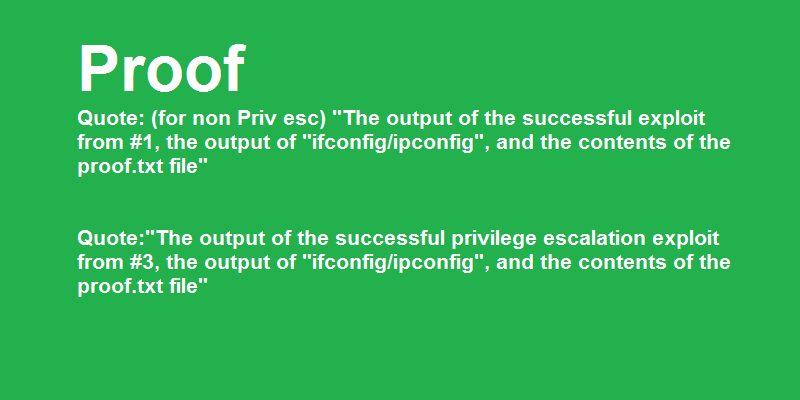
\includegraphics [width=\textwidth]{./hosts/\hostname/proof.png}
%scale 0.5 bedeutet 50% der originalgröße
%angle=90 Grafik um 90° drehen
\caption[Proof of \hostname]{Proof of \hostname} \label{\hostname-4}
\end{figure}


%---------------------End of host file
